\documentclass{ifacconf}
\usepackage[ruled,vlined,linesnumbered]{algorithm2e}
\usepackage{graphicx}
\usepackage[dvips]{epsfig}
\usepackage{epsf}
\usepackage{times}
\usepackage{xspace}
\usepackage[shortcuts]{extdash}
\usepackage{amsmath,amssymb}
\usepackage{amsfonts}
\usepackage{tabularx}
\usepackage{times}
%
\newtheorem{problem}{Problem}
\newtheorem{definition}{Definition}
\newtheorem{example}{Example}
\newtheorem{proposition}{Proposition}
%
\graphicspath{{figures/}}
%
% LaTeX macros
\newcommand{\sd}{\ensuremath{\mathrm{SD}}\xspace}
\newcommand{\dproblem}{\ensuremath{\mathrm{DP}}\xspace}
\newcommand{\comps}{\ensuremath{\mathrm{COMPS}}\xspace}
\newcommand{\obs}{\ensuremath{\mathrm{OBS}}\xspace}
\newcommand{\pr}{\ensuremath{\mathrm{Pr}}\xspace}
\newcommand{\ok}{\ensuremath{\mathrm{OK}}\xspace}
\newcommand{\inj}{\ensuremath{\mathrm{Inj}}\xspace}

%
\begin{document}
%
\begin{frontmatter}
%
\title{Model-Based Diagnosis Using Component Model Ensembles\thanksref{footnoteinfo}}
%
\thanks[footnoteinfo]{Supported by SFI grant 12/RC/2289.}
%
\author[First]{Alexander Feldman}
\author[First]{Johan de Kleer}
\author[Second]{Gregory Provan}
%
\address[First]{PARC Inc., Palo Alto, CA 94304 (e-mail: \{afeldman,dekleer\}@parc.com)}
\address[Second]{Department of Computer Science, University College Cork, Cork, Ireland (e-mail: g.provan@ cs.ucc.ie).}
%
\begin{abstract}
@todo
\end{abstract}
\end{frontmatter}
%
\section{Introduction}
%
Model-based diagnosis \cite{dekleer87diagnosing} uses system models
and sensor data to compute diagnostic hypotheses. These hypotheses
have a range of applications such as decision-making
\cite{feldman13genius}, repair, reconfiguration, troubleshooting,
testing, and many others. While providing many benefits, model-based
diagnosis is expensive due to the need of good system models. To
amortize this high modeling cost, researcher develop and use component
libraries.
\par
A component may have several representations in a component
library. For example, a NAND-gate may be model as a system of
non-linear equations that govern the analogue electrical laws of the
gate, or its linear approximation or with the simple Boolean
expression $o \leftrightarrow \neg(i_1 \wedge i_2)$. Although one may
say that the best choice of a component model is the one that
represents physics best (in the case of the NAND-gate, this would be
the analogue electrical model), experiments show that the result of
this choice is sometimes hard to predict and dependent on the
diagnostic context (i.e., on the use of the component models in the
final model).
\par
At present, to the best of our knowledge, there is no formal framework
for successfully generating a model of the ``correct'' fidelity. The
most common approach is to manually test different models to examine
trade-offs.
\par
In this article we propose the novel approach of using component model
ensembles consisting of multiple models of differing fidelity, for
diagnostics inference. Model ensembles have been used successfully in
machine learning \citep{brown2010ensemble,dietterich2000ensemble}, but
have not been adopted in diagnostics inference.
\par
The main idea of this article is to use a test-set of diagnostic
scenario for learning the optimal system model. The test-cases in the
test-set can be artificially generated (e.g., by simulation) and
contain a representative set of likely faults. The algorithm we
propose chooses these component models that optimize some (weighted)
diagnostic metrics such as diagnostic accuracy (which is dual of
classification errors), isolation time, or computational complexity
\cite{feldman10empirical}. The output of the algorithm is a system
model composition that can be later used unsupervised.
\par
To illustrate the usability of our algorithm, consider the diagnostic
model of a crane. The model would likely contain parts such as
electrical motors and drives and a Programmable Logic Controller
(PLC). Clearly, non-linear electromechanical-models are most
appropriate for the choice of the moving parts, however modeling the
PLC with non-linear equations would result in a suboptimal diagnosis
due to high complexity. Further, high simulation accuracy does not
necessarily translate to high diagnostic accuracy. The algorithm we
propose would run a few diagnoses and would discard the high-fidelity
PLC model to use the computationally simpler
Boolean/qualitative/state-machine components.
\par
We illustrate the working of our algorithm on a dynamic system used
widely in literature. This system consists of three tanks connected
with valves. Even for such small system the output of the algorithm is
non-intuitive. Last, the experiments in this paper make us believe
that the choice of modeling abstraction depends to a large extent on
the model topology and cannot be preconceived during the design of the
component library.

%************************************************************************
\section{Related Work}
\label{sec-RelWork}
%************************************************************************
Model ensemble methods have been applied in disciplines ranging from statistics
to AI (e.g.,~\citep{breiman1996stacked,clemen1989combining,perrone1992soft,wolpert1992stacked}),
and it has been shown that an ensemble is often more accurate than any single
model in the ensemble~\citep{maclin2011popular}.

The idea behind model ensemble is to build a predictive model by integrating multiple models to achieve better performance than could be obtained from the individual ones~\citep{maclin2011popular,rokach2010ensemble}. Roughly speaking, an ensemble
method is a supervised learning-based approach to discover which combination of
model has the best predictive power~\cite{kuncheva2003measures}.

The most popular ensemble algorithms are Bagging and Boosting, which are meta-algorithms
that pool decisions from multiple classifiers.
%
Proposed in 1996 by Leo Breiman, Bagging~\citep{breiman1996stacked}, which stands for
Bootstrap Aggregating, is a \textit{bootstrap}-based ensemble method~\citep{efron1994introduction}.
It applies a majority vote from classifiers trained on bootstrap samples (obtained by
random sampling with replacement) of the training data.

Boosting~\citep{freund1996experiments,schapire1990strength} iteratively learns weak
classified; producing a weighted sum of the results of weak classifiers. The training set
used for each member of the series is chosen based on the performance of the earlier
classifiers in the series. Note that, conversely to Boosting, the resampling of the
training set in Bagging is not dependent on the performance of the earlier classifiers.
Many different kinds of boosting algorithms have been proposed in the past: the
award winning Adaboost: Adaptive boosting~\citep{freund1996experiments}; LPBoost:
Linear Programming Boosting~\citep{demiriz2002linear} is a margin-maximizing classification
algorithm with boosting; BrownBoost~\cite{freund2001adaptive} is a boosting algorithm
that may be robust to noisy datasets; and LogitBoost~\cite{friedman2000additive} approach
which casts the AdaBoost algorithm into a statistical framework.

To the best of our knowledge, model ensemble methods have not been applied to
diagnostics before.

In the context of software fault localization using spectrum-based fault
localization~\citep{abreu2007accuracy}, approaches have been proposed to combine
several heuristics. In~\citep{wang2011search} a search-based algorithm to combine
the existing heuristics. In~\citep{xuan2014learning}, it is proposed a machine
learning-based approach to combine multiple diagnostic rankings metrics. An approach
based in data fusion to heuristic combination was proposed in~\citep{lo2014fusion}.

Another body of related work is research related to choosing the right level of
modeling abstraction. As an example, in the model-based diagnosis literature,
there has been considerable work on diagnostic assumptions and selecting appropriate
models for a diagnostic task~\citep{struss1992s}. The work proposed in~\citep{de2007dynamic}
focuses primarily on assumptions associated with choosing domain abstractions.

There has been considerable research on structural abstraction~\citep{chittaro2004hierarchical,hamscher1990xde}
where groups of components are combined to form larger systems to reduce computational
complexity. The work in~\citep{sachenbacher2005task} describes how the task can be
used to partition the value of a variable into the qualitative values needed to solve a
task. In~\citep{torta2003automatic} presents another
approach to partition the value of a variable into qualitative ranges to reduce
complexity when there is limited observability of the variables.

TODO: we need a sentence on why this is different.

\section{Concepts and Definitions}\label{sec:concepts}
%
All concepts, definitions, and algorithms discussed in this article
are illustrated on a commonly used dynamic system consisting of water
tanks that are connected with valves.
%
\subsection{Running Example}
%
The three-tank system is shown in figure~\ref{fig:three_tanks}. The
tanks are denoted as $T_1$, $T_2$, and $T_3$. They all have the same
area $A_1 = A_2 = A_3 = 3~[\textrm{m}^2]$. The three tanks are
indestructible and of infinite height representing an idealized
experiment.  We assume that $g = 10$ and the liquid is ``pure'' water
with density $\rho = 1$.
%
\begin{figure}[htb]
  \centering
  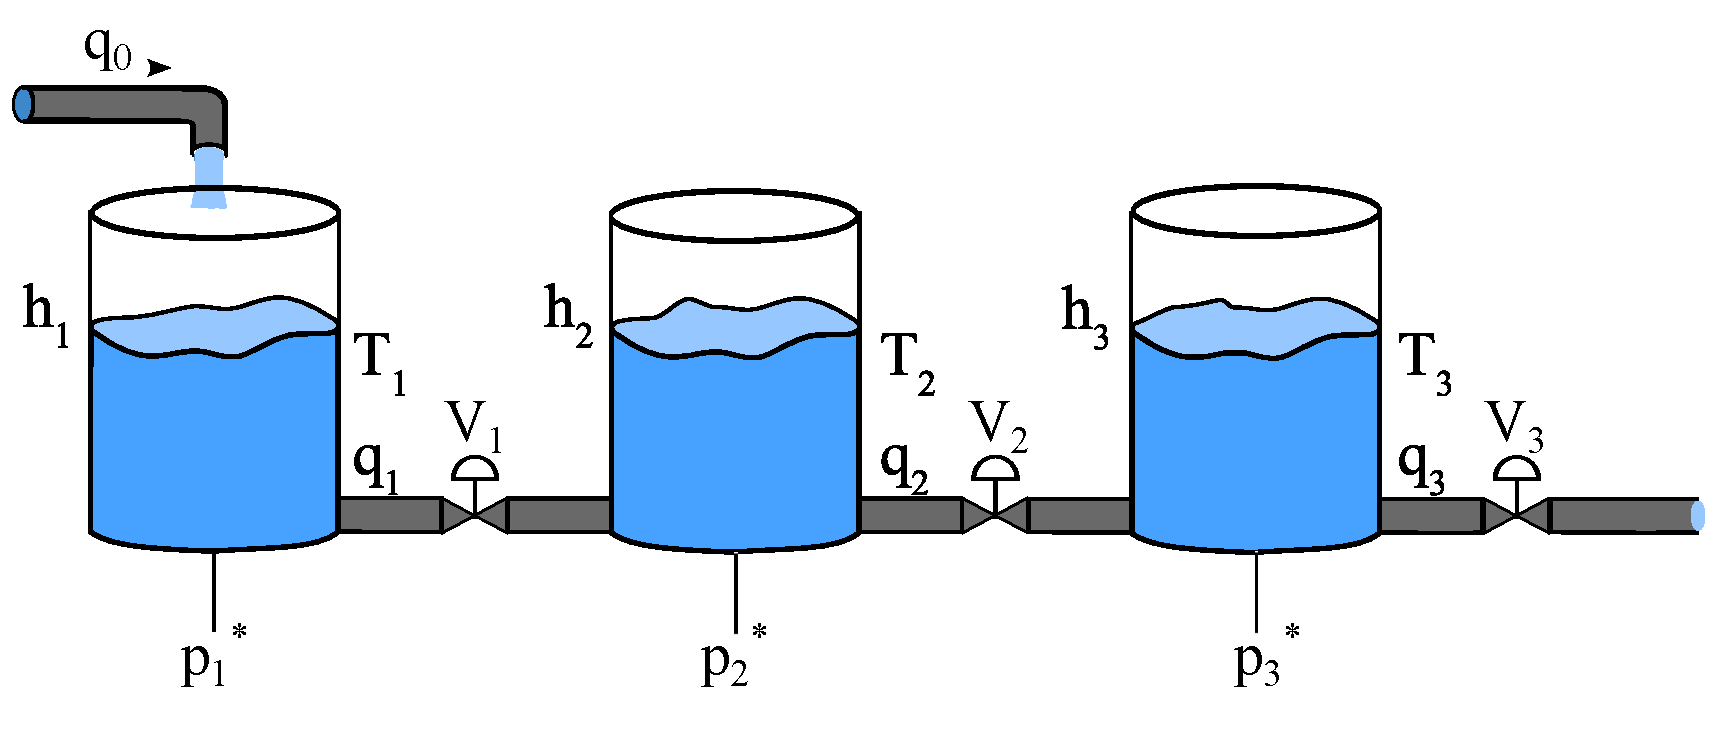
\includegraphics[width=1\columnwidth]{3-tanks}
  \caption{Diagram of the three-tank system.}
  \label{fig:three_tanks}
\end{figure}
\par\noindent
%
Tank $T_1$ is filled from a pipe $q_0$ with a constant flow of
$0.75~[\textrm{m}^3/\textrm{s}]$. It drains into $T_2$ via a pipe
$q_1$. The liquid level is denoted as $h_1$. There is a pressure
sensor $p_1$ connected to $T_1$ that measures the pressure in Pascals
[Pa]. Starting from Newton's (and Bernouli's) equations and
manipulating them (the actual derivation is irrelevant in this paper)
we derive the following Ordinary Differential Equation (ODE) that
gives the level of the liquid in $T_1$:
%
\begin{eqnarray}
%
\frac{d h_1}{dt} = \frac{q_0 - k_1 \sqrt{h_1 - h_2}}{A_1}\label{eq:ode1}
%
\end{eqnarray}
%
In eq.~\ref{eq:ode1}, the coefficient $k_1$ is the product of the
cross-sectional area of the tank $A_1$ and the area of the drainage
hole and $\sqrt{2g}$ and the friction/contraction factor of the
hole. We emphasize the use of $k_1$ because, later, we will be
``diagnosing'' our system in term of changes in $k_1$. Consider a
physical valve $R_1$ between $T_1$ and $T_2$ that constraints the flow
between the two tanks. We can say that the valve changes
proportionally to the cross-sectional drainage area of $q_1$ and hence
$k_1$. The diagnostic task is to compute the true value of $k_1$,
given $p_1$, and from $k_1$ we can compute the actual position of the
valve $R_1$.
%
The water levels of $T_2$ and $T_3$, denoted as $h_2$ and $h_3$
respectively, are given by:
%
\begin{eqnarray}\label{eq:tank1}
%
\frac{d h_i}{dt} = \frac{k_{i - 1} \sqrt{h_{i - 1} - h_i} - k_i \sqrt{h_i}}{A_i},
%
\end{eqnarray}
%
where $i$ is the tank index ($i \in \{2, 3\}$).
\par
Let us say that $k_1 = k_2 = k_3 = 0.75$.
\par
Finally, we turn the water level into pressure:
\begin{eqnarray}
p_i = \frac{g\,h_i\,A}{A} = g\,h_i\label{eq:pressure}
\end{eqnarray}
where $i$ is the tank index ($i \in \{1, 2, 3\}$).
\par
It is assumed that the initial water level in the three tanks is zero.
%
Let us continue with some notation and definitions.
%
\subsection{Compositional Modeling}
%
Consider a component library $\cl = \left\{C_1, C_2, \ldots,
C_n\right\}$ where each component $C_i$ for $i = \left\{1, 2, \ldots,
n\right\}$ is defined as \textit{a set} of models. Each set $C_i =
\left\{C_{i, 1}, C_{i, 2}, C_{i, 3}\right\}$ contains a non-linear,
linear, and qualitative model describing the behavior of the $C_i$
component.

\begin{definition}[Non-Linear Model]
We write the dynamic equations for a model in state-space form using
\begin{eqnarray}\label{eq:nonlinear}
\dot{\vec{x}}(t) & = & \psi (\vec{x}(t)) + \vec{u}(t))\\
\vec{y}(t) & = & \gamma (\vec{x}(t)), \vec{u}(t)),
\end{eqnarray}
where $\psi$ and $\gamma$ are non-linear functions.
\end{definition}
%
In the case of the three-tanks example, the non-linear model of $T_1$
is given by equations (\ref{eq:ode1}) and (\ref{eq:pressure}) and the
models of $T_2$ and $T_3$ are given by equations (\ref{eq:tank1}) and
(\ref{eq:pressure}).
%
\begin{definition}[Linear Model]
We write the linear dynamical equations for a model in state-space form using
\begin{eqnarray}\label{eq:linear}
\dot{\vec{x}}(t) & = & \mathbf{A} \vec{x}(t) + \mathbf{B} \vec{u}(t) + \mathbf{C} \vec{\omega}(t) +  \vec{\omega}(t)\\
\vec{y}(t) & = & \mathbf{D} (\vec{x}(t)),
\end{eqnarray}
where $\mathbf{A}, ~ \mathbf{B},~\mathbf{C}$ and $\mathbf{D}$ are linear matrices.
\end{definition}
%
For the linear three-tank model we replace the non-linear sub-function
$\sqrt{h_{i - 1} - h_i}$ with the linear sub-function $\gamma_i (h_{i
- 1} - h_i)$, where $\gamma_i$ is a parameter (to be estimated)
governing the flow between tanks $i - 1$ and $i$. We obtain the
following system equations for tanks $T_2$ and $T_3$:
%
\begin{eqnarray}\label{eq:lineartank}
%
\frac{d h_i}{dt} = \frac{k_{i - 1}(h_{i - 1} - h_{i}) - k_i {h_i}}{A_i},
%
\end{eqnarray}
%
\begin{definition}[Qualitative Model]
We write the dynamical equations for a model in state-space form using
\begin{eqnarray}\label{qual-model}
\dot{\vec{x}}(t) & = & \upsilon (\vec{x}(t)) + \vec{u}(t))\\
\vec{y}(t) & = & \mu (\vec{x}(t)), \vec{u}(t)),
\end{eqnarray}
where $\upsilon$ and $\mu$ are functions from the set of reasonable
functions $f$ such that $f' > 0$ on the interior of its domain
\citep{kuipers1994composition}.
\end{definition}
%
For the qualitative model we replace the non-linear sub-function
$\sqrt{h_{i - 1} - h_i}$ with the qualitative $M^+(h_{i - 1} - h_i)$,
where $M^+$ is the set of reasonable functions $f$ such that $f' > 0$
on the interior of its domain
\citep{kuipers1994composition}.
%
\begin{eqnarray}
%
\frac{d h_i}{dt} = \frac{1}{A_2}\left[\kappa_{1} M^+(h_{i} - h_{i - 1}) - \kappa_2 M^+(h_i)\right]
%
\end{eqnarray}
%
The tank heights are constrained to be non-negative. As a consequence,
we can discretize the $h_i$ to take on values $\{+, 0\}$, which means
that $M^+(h_i)$ can take on values $\{+, 0, -\}$.  The domain for
$\frac{d h_1}{dt}$ must be $\{+, 0, -\}$, since $q_0$ is non-negative
and each $M^+(h_i - h_j)$ can take on values $\{+, 0, -\}$.
\par
A decomposable model can be described using two orthogonal aspects:
\textit{behavior} and \textit{topology} (interaction). The behavior
model describes the (possibly dynamic) behaviors of the system and
components. The topology model describes component connectivity in
terms of components and their connections, and defines the constraints
on component behaviors that enable their interactions to be specified
at the system-level.
\par
The topology of a system describes how the components are connected.
%
\begin{definition}[Topology]
%
We describe the system topology of a composable system using a graph
$G(V, E)$, where vertices $V$ correspond to components and edges in
$E$ correspond to connections between components.
%
\end{definition}
%
\begin{definition}[System Description]
%
Given a component library \cl, a topology $G(V, E)$, and some law of
composition $\mathcal{L}$, a system description $\sd = \langle\Phi,
\comps, \obs\rangle$ is defined as a set of
equations $\Phi$, a set of component variables $\comps$, and a set of
observable variables $\obs$.
%
\end{definition}
%
%\begin{definition}
%
%A composable system $\Psi$ is defined using the pair $(G,{\Phi})$,
%where $G$ is the topology model and ${\Phi}$ is the behavior model.
%
%\end{definition}
%
%
%We assume a (simulation) model to consist of a set of equations $\Phi$
%describing the behavior of a system model.
%\par
%In this article we examine several different types of model for
%simulation, including dynamical, linear, and qualitative. For our
%models, we consider three classes of variables: $\vec{x}(t)$ is the
%state variable vector, $\vec{u}(t)$ is the input variable vector, and
%$\vec{y}(t)$ is the output vector. We assume that the output of a
%system can be observed in which case we denote the set of observable
%variables as $\obs = \vec{y}(t)$. In addition to that,
%$\vec{\omega}(t)$ is a disturbance vector.

\subsection{Diagnostic Problem}
%
\begin{definition}[Observation]
%
Given a system description \sd, an observation $\tilde\alpha =
\langle\alpha, t_{\mathrm{obs}}\rangle$ is an instantiation of the
variables in \obs at a time instant $t_{\mathrm{obs}}$.
%
\end{definition}
%
One possible observation for our running example is:
$p_1 = 142.4$, $p_2 = 26.8$, and $p_3 = 13$ at $t_{\mathrm{obs}} =
300$.
%
\begin{definition}[Fault Injection]
%
Given a system description \sd, a fault injection $\tilde{\varepsilon}
= \langle\varepsilon, t_{\mathrm{inj}}\rangle$ is an instantiation of
the variables in \comps at a time instant $t_{\mathrm{inj}}$.
%
\end{definition}
%
For the three-tanks example, fault injection values of $R_1 = 0.5$ at
time $t_{\mathrm{inj}} = 250$ would correspond to the first valve
being stuck at $50\%$.
%
\begin{definition}[Diagnosis]\label{def:diagnosis}
%
Given a system description \sd, a diagnosis $\tilde{\omega} =
\langle\omega, t_{\mathrm{diag}}\rangle$ is a probabilistic assignment
of the variables in \comps at a time instant $t_{\mathrm{diag}}$.
%
\end{definition}
%
Continuing with the example, a diagnosis that reflects the given
observation and non-linear model of the three tanks is $\pr(R_1 =
0.931)$ at time $t_{\mathrm{diag}} = 310$ which isolates the fault in
$60$ s with high accuracy.
\par
All above definitions are used in formulating the main diagnostic
problem for dynamic systems:
%
\begin{definition}[Diagnostic Problem]
%
A diagnostic problem \dproblem is defined as the quadruple $\dproblem
= \langle\sd, \tilde{\alpha}, \tilde{\varepsilon},
\tilde{\omega}\rangle$.
%
\end{definition}
%
Before we propose how to solve diagnostic or inverse diagnostic
problems, we need a method for evaluating the performance of a
diagnostic algorithm.
%
\subsection{Diagnostic Performance Metrics}
%
Unlike other AI disciplines, in MBD there are multiple factors that
should be considered when applying performance metrics to real-world
systems. The most important computational metric is the number of
diagnostic errors which is dual to the isolation accuracy
\citep{feldman10empirical}.
%
\begin{definition}[Diagnostic Errors]
%
Given a diagnostic problem \dproblem the diagnostic errors metric
$M_{\mathrm{err}}$ is defined as:
%
\begin{eqnarray}
%
M_{\mathrm{err}} = \sum_{c \in \comps}{\left|\pr(\omega_c \ne \ok) - \inj(\varepsilon_c)\right|}
%
\end{eqnarray}
%
\end{definition}
%
The second most important metric for a dynamic system is the time
between a fault is injected and when the algorithm detects a fault.
%
\begin{definition}[Isolation Time]
%
Given a diagnostic problem \dproblem the isolation time metric
$M_{\mathrm{iso}}$ is defined as:
%
\begin{eqnarray}
%
M_{\mathrm{iso}} = t_{\mathrm{diag}} - t_{\mathrm{inj}}
%
\end{eqnarray}
%
\end{definition}
%
Diagnostic algorithms are typically given a system model \sd and a set
of test cases $\mathcal{A} = \left\{\langle\tilde\alpha_1,
\tilde\varepsilon_1\rangle, \langle\tilde\alpha_2,
\tilde\varepsilon_2\rangle, \cdots, \langle\tilde\alpha_n,
\tilde\varepsilon_n\rangle\right\}$. The main goal of these diagnostic
algorithms is to optimize a superposition of the diagnostic
metrics. Each diagnostic metric is weighted with a domain specific
coefficient (these are $g_{\mathrm{err}}$, and $g_{\mathrm{iso}}$,
respectively, in the the cases of $M_{\mathrm{err}}$, and
$M_{\mathrm{iso}}$). In this article, however, we solve an orthogonal
problem: given a diagnostic algorithm, a component library and a set
of test cases $\mathcal{A}$, compute a model composition \sd such that
$g_{\mathrm{err}}M_{\mathrm{err}} + g_{\mathrm{iso}}M_{\mathrm{iso}}$
is minimized.

\section{Ensemble Learning Algorithm}
%
The main idea of this paper is shown in
algorithm~\ref{alg:compose_model}. This is a high-level description
and the algorithm uses a diagnostic engine similar to the one
described by \cite{feldman13genius}.
%
\begin{algorithm}[htb]
\begin{footnotesize}
%
\caption{\textsc{ComposeModel}($T, \mathcal{C}, \mathcal{A}$)}
\label{alg:compose_model}
%
\KwIn{$T$, model topology}
\KwIn{$\mathcal{C}$, component library}
\KwIn{$\mathcal{A}$, set of test scenarios}
\KwResult{\sd, model}
%
\SetKwInput{KwLocals}{Local variables}
\SetKwInput{KwLocal}{Local variable}
\KwLocals{$\sd^\star$, $\sd^\prime$, models, initially $\emptyset$}
\KwLocal{$\alpha$, test scenario}
\KwLocal{$\omega$, diagnosis}
\KwLocal{$m$, diagnosis score}
\KwLocal{$m_{\min}$, optimal diagnosis score, initially $\infty$}
%
\vspace{0.075in}
%
\Repeat
{
$\textsc{Terminate?($\sd^\star, \sd^\prime, m$)}$
}
{
    $\sd^\star \gets \textsc{NextModelComposition}(T, \mathcal{C}, \sd^\prime)$\label{alg:next_model_composition}\\
    $\sd^\prime \gets \sd^\star$\\
    $m \gets 0$\\
    \ForEach{$\alpha \in \mathcal{A}$}
    {
        $\omega \gets \textsc{Diagnose}(\sd^\star, \alpha)$\\
        $m \gets m + \textsc{Evaluate}(\alpha, \omega)$\label{alg:evaluate}\\
    }
    \If{$m < m_{\min}$\label{alg:accept_start}}
    {
        $m_{\min} \gets m$\\
        $\sd \gets \sd^\star$\label{alg:accept_end}\\
    }
}
\textbf{return} $\sd$
%
\end{footnotesize}
\end{algorithm}
%
\par
%
Algorithm~\ref{alg:compose_model} is presented as
non-deterministic. The non-determinism is in the auxiliary function
\textsc{NextModelComposition}
(line~\ref{alg:next_model_composition}). This function takes a model
topology and a component library as inputs and returns a composed
model. Each component has multiple representations in the component
library (e.g., qualitative, linear, non-linear). The total number of
component combinations is, of course, $n^{|\comps|}$, where $n$ is the
number of representations. Fortunately, there is no need to perform a
complete-search over the space of all possible model compositions. A
greedy-search strategy achieves satisfactory performance in most
practical cases.
\par
A configuration of algorithm~\ref{alg:compose_model} that determines
many of the diagnostic performances is the order in which
health-assignments are generated. This is implemented in the
\textsc{NextModelComposition} function. The
\textsc{NextModelComposition} subroutine also determines when to stop
the search and should be properly parametrized depending on the model
and the user requirements. In our implementation we provide the
following model-composition search policies:
%
\begin{description}
%
\item[Breadth-First Search (BFS):]
{
%
This search policy starts with all components having the same model
types (for example non-linear), then considers all models with a
single component type change. After all single component type changes
are exhausted, the algorithm continues with pairs of components,
triples, etc.
%
}
\item[Depth-First Search (DFS):]
{
%
The algorithm starts by changing the type of the first component, then
the second, etc., until all component types are changed. At this
point, algorithm~\ref{alg:compose_model} backtracks one step,
generates a sibling assignment and continues traversing down and
backtracking in the same manner until no more backtracking is
possible.
%
}
\item[Forward Greedy Stochastic Search (FGSS):]
{
%
This is a randomized search policy. In this mode, the algorithm starts
by changing the type of one of the components. If the change improves
the metric in line~\ref{alg:evaluate} of
algorithm~\ref{alg:compose_model}, then the change is accepted (see
lines~\ref{alg:accept_start}--\ref{alg:accept_end} of
algorithm~\ref{alg:compose_model}). This is our preferred search
policy as typically the evaluation metric improves monotonically when
changing the component types one by one.
%
}
\item[Backwards Greedy Stochastic Search (BGSS):]
{
%
In this mode, the search start from all component types changed from
their defaults. The type of a random component is then flipped and the
flip is retained iff the flip leads to a decrease in total metric
evaluation score. The order of component is arbitrary. As the whole
search process is stochastic, it needs to be run multiple iterations
in order to achieve the desired completeness.
%
}
%
\end{description}

%************************************************************************
\section{Empirical Analysis}
%************************************************************************

\subsection{Experimental Design}

For each of the 3 model types, we define sub-models incorporating weak- and strong-fault variants. This leads to an ensemble of 6 models.

For each of a collection of ${\cal A} = \{\vec{\alpha}\}$ of system observations, we compute diagnoses and average them.
\section{Conclusions}\label{sec:conclusions}
%
Despite successful applications within the machine learning community~\citep{brown2010ensemble,dietterich2000ensemble},
model ensembles have not been adopted in diagnostics inference. This paper addresses that gap by proposing
an algorithm that, given a test set of diagnostic scenarios, learns the optimal system model from a library of component
models.

We have shown the proposed algorithm on a dynamic system consisting of three tanks connected with valves. Results
indicate that the model composition may be non-intuitive and suggest that the choice of modeling abstraction depends
on the model topology and cannot be preconceived during the design of the component library.

Future work includes a thorough validation of the proposed algorithm using different topologies, modeling abstraction
libraries, and different fault scenarios. We are also interested in investigating the impact of the learning phase
in the detection phase of the algorithm.

%
\bibliography{safeprocess15-ensembles}
%
\end{document}
